\documentclass{article}
\usepackage[utf8]{inputenc}
\usepackage{amsmath, amsthm, mathtools, amsfonts, graphicx, hyperref,setspace, xparse, algorithm, algpseudocode, mathabx}

\addtolength{\oddsidemargin}{-0.5in}
\addtolength{\evensidemargin}{-0.5in}
\addtolength{\textwidth}{1in}

\usepackage{biblatex, tikz}
\addbibresource{bibliography.bib}

\theoremstyle{plain}% default
\newtheorem{theorem}{Theorem}[section]
\newtheorem{lemma}[theorem]{Lemma}
\newtheorem{prop}[theorem]{Proposition}
\newtheorem{ppties}[theorem]{Properties}
\newtheorem{cor}{Corollary}
\theoremstyle{definition}
\newtheorem{definition}{Definition}[section]
\newtheorem{example}{Example}[section]
\newtheorem{numexmp}{Numerical Example}[section]
\theoremstyle{remark}
\newtheorem*{remark}{Remark}
\newtheorem*{note}{Note}
\newtheorem{case}{Case}

%\title{Hamiltonian Monte Carlo and Common Random Number}
\title{Common Random Number applied to examples}
\author{Sabrina Sixta}
\def\mc{Markov chain }
\def\sumn{\sum_{i=1}^n}
\def\andd{\bigcap}
\def\orr{\bigcup}
\def\io{\;\; i.o.}
\def\lfa{\leftrightarrow}
\def\ls{\lambda_*}
\def\wrt{with respect to }
\def\limn{\lim_{n\to \infty}}
\def\fld{\mathcal{F}}
\def\inn{\subseteq}
\def\supa{\sup_{A \subseteq S}}
\def\qd{q(\cdot,\cdot)}
\def\sump{\sum_{i=1}^p}
\def\vecx{\vec{X}}
\def\L{\mathcal{L}}
\def\X{\mathcal{X}}
\def\bbX{\boldsymbol{\X}}
\def\mcxn{\{X_n\}_{n\geq 1}}
\def\N{\mathbb{N}}
\newcommand{\indep}{\perp \!\!\! \perp}
\def\tin{\tau^{-1}}
\def\G{\Gamma}
\def\ax{p/2}
\def\bx{C/2}
\def\ay{(k+p)/2}
\def\by{C/2}
\def\tinv{\tau^{-1}}
\def\aax{1/2}
\def\bbx{S/2}
\def\aay{(J+2)/2}
\def\bby{S/2}
\def\borel{\mathcal{B}}

\doublespacing

\begin{document}
	\maketitle
	
	\section{Convergence rate of CRN and backward processes are the same}
	Define a Markov chain $\{X_n\}_{n\geq 1}$ in $(\mathcal{X},\mathcal{F})$ such that $X_n = f_{\theta_n}(X_{n-1})$, where  $\{\theta_n\}_{n\geq 1}$ are i.i.d. random variables on some measurable space $\Theta$ and random measurable mappings $f_{\theta_n} : \mathcal{X} \mapsto \mathbb{R}$. The set of random functions $f_{\theta_1}, f_{\theta_2},\ldots$ is called an iterated function system. Any time-homogeneous Markov chain can be represented as an iterated function system \cite{avcont}.
	
	The iterated function system defines the forward and backward processes. The forward process, $\{X_n\}_{n\geq 1}$, which is a Markov chain, is defined as follows,
	$$X_n = f_{\theta_n}(f_{\theta_{n-1}}(\ldots f_{\theta_1}(X_0)))$$
	
	The backward process, $\{\tilde{X}_n\}_{n\geq 1}$, which is not a Markov chain \cite{localcont} with respect to filtration for $X_0, \ldots, X_n$ but tends to converge pointwise to a limit, is defined as follows,
	$$\tilde{X}_n = f_{\theta_1}(f_{\theta_{2}}(\ldots f_{\theta_n}(X_0)))$$
	
	Figure \ref{fig:backwardsvsforwards} graphs the forward and backward process of an autoregressive normal process using the same random mappings. The point towards which the backwards process converges is itself random. 
	
	\begin{figure}
		\centering
		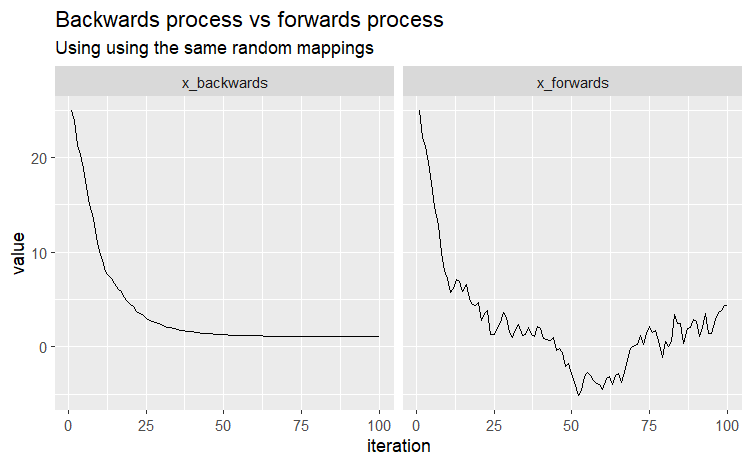
\includegraphics[width=0.7\linewidth]{images/backwardsvsforwards}
		\caption{The backwards, $\{\tilde{X}_n\}_{n\geq 1}$, and forwards, $\{X_n\}_{n\geq 1}$, process of the autoregressive normal system where $X_n,\tilde{X}_n$ are simulated using the same random mappings, $X_n=0.9X_{n-1}+Z_n, Z_n\sim N(0.1)$ and $X_0=25$.}
		\label{fig:backwardsvsforwards}
	\end{figure}
	
	Despite the difference in behaviour of the two processes, the marginal distributions of the forward and backward processes are the same, $X_n \overset{d}{=}\tilde{X}_n$, so the backwards process is sometimes used when studying convergence properties of the forwards Markov chain \cite{iteratedranfunc,avcont,localcont}.
	
	%	When studying the convergence rates of iterated random functions, we are typically interested in establishing a contraction condition. The `vanilla' contraction condition, sometimes referred to as global average \cite{avcont} or strongly \cite{localcont} contractive, is defined as the supremum over all $x$ of the expected Lipschitz constant. 
	%	
	%	\begin{definition}[Global average contraction condition]\label{def:cont}
		%		An iterative function system is global average contractive if there exists a $D\in (0,1)$ such that, $$D \geq \sup_{x \not= x'} \frac{E[d(f_{\theta}(x),f_{\theta'}(x'))]}{d(x,x')}$$
		%	\end{definition}
	%	
	%	Modifications to the above contraction condition have been widely studied and can be found in \cite{iteratedranfunc, ifssurvey, tweedielocalcont, ifssurvey1, localcont, avcont}. 
	
	\begin{theorem}
		%Given two forward processes $X_n, X'_n$ that are simulated using the CRN technique (i.e., $X_n=f_{\theta_n}(X_{n-1})$ and $X'_n=f_{\theta_n}(X'_{n-1})$ for $n\in \mathbb{N}$), and the corresponding backwards process $\tilde{X}_n$, 
		The expected distance between the $n$th iteration of the two forward processes where $X_0=x$ and $X'_0=f_{\theta_{n+1}}(x)$ is equal to the expected distance between the $n$th and $(n+1)$th iteration of the backwards process, $\tilde{X}_n$. 
		
		$$E[d(X_n,X'_{n})\mid X_0=x, X'_{0}=f_{\theta_{n+1}}(x)]=E[d(\tilde{X}_n,\tilde{X}_{n+1})\mid \tilde{X}_0 = x]$$
		
		\begin{proof}
			\begin{align*}
				&E[d(X_n,X'_{n})\mid X_0=x, X'_{0}=f_{\theta_{n+1}}(x)] \\
				&=E[d[f_{\theta_n}(f_{\theta_{n-1}}(\ldots f_{\theta_1}(x)\ldots)),f_{\theta_n}(f_{\theta_{n-1}}(\ldots f_{\theta_1}(f_{\theta_{n+1}}(x))\ldots))]\mid X_0=x]\\
				&=E[d[f_{\theta_1}(f_{\theta_{2}}(\ldots f_{\theta_n}(x)\ldots)),f_{\theta_1}(f_{\theta_{2}}(\ldots f_{\theta_n}(f_{\theta_{n+1}}(x))\ldots))]\mid \tilde{X}_0=x]\\
				&= E[d(\tilde{X}_n,\tilde{X}_{n+1})\mid \tilde{X}_0 = x]
			\end{align*}
		\end{proof}
	\end{theorem}
	
	
	\section{Sufficient conditions for when CRN converges a.s. when there is convergence in distribution}
	
	The following is a theorem that we will use to prove that random variables simulated according to common random number converge almost surely. We've adjusted the theorem notation to describe distribution functions.
	\begin{prop}[Theorem 2 of \cite{invconv}]\label{thm:invconvgen}
		Let  $\{F_n\}_{n\geq 0}$ be a sequence of mappings. If
		\begin{enumerate}
			\item $\{F_n\}_{n\geq 0}$ is a sequence of injective mappings on a metric space
			$(\mathbb{R}^d,||^2)$ and taking values in a locally compact metric space $([0,1],||)$,
			\item $F_n\to F$ uniformly on $\mathbb{R}^d$, 
			\item $F^{-1}$ is a continuous mapping on $[0,1]$
		\end{enumerate}
		Then $F^{-1}_n\to F^{-1}$ uniformly on every compact set $K_0$ contained in $N_0=Interior[0,1]\cap_{n\geq 1}Im(F_n)$
	\end{prop}
	
	Theorem \ref{thm:invconvgen} is a general theorem, but we are only interested in the theorem applied to distribution functions. Many of the requirements are already fulfilled for distribution functions (for example if $F_n\to F$ and $F$ is continuous then the convergence is uniform (see example 14.8 of \cite{billingsley}, theorem 1.1 of \href{https://researchers.ms.unimelb.edu.au/~xgge@unimelb/Files/Teaching/Advanced%20Probability%20(Semester%201%202020)/Lecture%20Notes.pdf}{this}), the metric space $([0,1],\lambda)$ is already locally compact, if $F^{-1}$ is continuous then $F$ is continuous \href{https://math.stackexchange.com/questions/541082/proving-the-inverse-of-a-continuous-function-is-also-continuous}{Why does Google always send me to mathStackExchange???} etc.), so we can rewrite theorem \ref{thm:invconvgen} as follows.
	
	\begin{prop}[Theorem 2 of \cite{invconv} adjusted for distribution functions]\label{thm:invconvgen}
		Let  $\{F_n\}_{n\geq 0}$ be a sequence of mappings. If
		\begin{enumerate}
			\item $\{F_n\}_{n\geq 0}$ is a sequence of strictly increasing distribution functions on a metric space
			$(\mathbb{R}^d,||^2)$ and taking values in $([0,1],||)$, 
			\item $F_n\to F$ on $\mathbb{R}^d$
			\item $F$ is a continuous, invertible mapping on $[0,1]$
		\end{enumerate}
		Then $F^{-1}_n\to F^{-1}$ uniformly on every compact set $K_0\in (0,1)$.
	\end{prop}
	
	\begin{definition}[Uniform convergence of functions]
		The given the sequence of functions $F_{n}:(\mathbb{R}^d,||^2)\to ([0,1],||)$ and the target function $F:(\mathbb{R}^d,||^2)\to ([0,1],||)$,  $F_n\to F$ uniformly if for all $\epsilon >0$, there exists an $N\in\mathbb{N}$ such that for any $n\geq N$ and $x\in \mathbb{R}^d$, 
		$$|F_n(x)-F(x)|\leq \epsilon$$
	\end{definition}
	
	This theorem implies the following result. Namely let $F$ be a target distribution function and 
	\begin{enumerate}
		\item $\{X_n(u)\}_{n\geq 1}$ be a sequence of random variables with $X_n(u)=F^{-1}_n(u)$, $F_n\to F$ on $\mathbb{R}^d$ and $F_n, n\geq 1$ is strictly increasing  on $\mathbb{R}^d$
		\item $\{X'_n(u)\}_{n\geq 1}$ be a sequence of random variables with $X'_n(u)=F^{'-1}_n(u)$, $F'_n\to F$ on $\mathbb{R}^d$ and $F_n, n\geq 1$ is  strictly increasing on $\mathbb{R}^d$
	\end{enumerate}
	
	Common random number simulation of $X_n, X'_n$, means that for each iteration $n$, we simulate $U_n\sim Unif(0,1)$ and generate the random variables, $X_n(U_n), X'_n(U_n)$, from the same $U_n$. 
	
	\begin{theorem}\label{thm:skorohod}
		Suppose that $X_n,X'_n$ are defined as above and the limiting distribution $F$ is a continuous, invertible mapping on $[0,1]$. If $X_n, X'_n$ are simulated according to common random numbers, then  $|X_n(U_n)-X'_n(U_n)|\to 0$ almost surely.
		
		\begin{proof}
			First note that conditions 1 and 2 of Proposition \ref{thm:invconvgen} are satisfied by the definitions of $X_n,X'_n$.
			
			Let $K_k=[\frac{1}{k}, 1-\frac{1}{k}]$, $k>2$ be a compact set. Then by definition of uniform convergence for any $\epsilon >0$, there exists an $N_1,N_2\in\mathbb{N}$ such that for any $n_1\geq N_1$ and $n_2\geq N_2$ and $u\in K_k$, 
			\begin{align*}
				|F^{-1}_{n_1}(u)-F^{-1}(u)|&\leq \epsilon/2\\
				|F^{'-1}_{n_2}(u)-F^{-1}(u)|&\leq \epsilon/2
			\end{align*}
			So for $n\geq \max\{N_1,N_2\}$,
			$$|F^{-1}_{n}(u)-F^{'-1}_{n}(u)|\leq |F^{-1}_{n}(u)-F^{-1}(u)|+|F^{'-1}_{n}(u)-F^{-1}(u)|\leq \epsilon/2+\epsilon/2=\epsilon$$
			This means that 
			$$P(\lim_{n\to\infty} |F^{-1}_n(u)-F^{'-1}_n(u)|\leq \epsilon)\geq P(U\in K_k)=1-\frac{2}{k}$$
			Since $k>2$ is arbitrary, we set $k\to\infty$ and so,
			$$P\left(\lim_{n\to\infty} |F^{-1}_n(u)-F^{'-1}_n(u)|\leq \epsilon\right)=P\left(\lim_{n\to\infty} |X_n(u)-X'_n(u)|\leq \epsilon\right)=1$$
		\end{proof}
	\end{theorem}
	
	\newpage
	\section{Necessary and sufficient conditions for CRN to generate the Wasserstein distance}
	\begin{prop}[Proposition 2.2 of \cite{crn} for $\theta \in \mathbb{R}$]\label{prop2}
		Fix $x, y \in \mathbb{R}$ and let $X=f(\theta_U,x)$ and $Y=f(\theta_V,y)$ with measurable $f : \mathbb{R}^2 \to \mathbb{R}$ where  $\theta_U = F^{-1}_{\theta}(U)$, $\theta_V = F^{-1}_{\theta}(V)$ and $U,V\sim Unif(0,1)$.
		Suppose for $z \in \{x,y\}$, $f(\cdot, z)$ is a non-decreasing continuous function with $E[X^2], E[Y^2] < \infty$. 
		Then
		\begin{equation}
			W(\mathcal{L}(X), \mathcal{L}(Y)) = \inf_{(X, Y) \sim J (X,Y)}E[(X-Y)^2]=E[(f(\theta_U,x)- f(\theta_U,y))^2]
		\end{equation}
		or
		\begin{equation}
			\sup_{(U, V) \sim J(U,V)} E[f(\theta_U,x)f(\theta_V,y)]
		\end{equation}
		is attained by setting $U = V$. 
	\end{prop}
	
	\textbf{The fundamental problem with extending this to $\mathbb{R}^d, d>1$ is that there is no practical ordering in $\mathbb{R}^d$. Both of the following claim that optimality cannot be extended to $\mathbb{R}^d$ in a practical way: \href{https://arxiv.org/pdf/1803.00567}{Remark 2.30} and \href{https://link.springer.com/book/10.1007/978-3-319-20828-2}{Chapter 2 of this}}
	
	
	\begin{theorem}\label{thm:crngen}
		For fixed $x, y \in \mathcal{X}$, let $X = f(\theta_U,x)$ and $Y = f(\theta_V,y)$ be random functions with measurable $f: \mathbb{R}^2 \mapsto \mathbb{R}$ and $\theta_U = F^{-1}_{\theta}(U)$ and $\theta_V = F^{-1}_{\theta}(V)$ with $U,V\sim Unif(0,1)$. 
		For $z \in \{x,y\}$, assume $\theta \mapsto f(\theta, z)$ is of bounded variation (see section 3.1 of \cite{realanalysis} for definition) and has finite second moments. 
		%Let $I_z$ be the area over which $\theta \mapsto f(\theta, z)$ is a non-decreasing function and $D_z$ is the area over which $\theta \mapsto f(\theta, z)$ is a non-increasing function.
		
		Let $I_z=\{\theta\mid f(\theta,z)\text{ is stochastically monotone}\}$ and $D_z=\{\theta\mid f(-\theta,z)\text{ is stochastically monotone}\}$
		Define the set $A =(I_x\cap I_y)\cup (D_x\cap D_y)$.
		
		\begin{itemize}
			\item If $P(A)=1$,% (the intervals of positive measure over which $\theta$ is increasing and decreasing on $f(\cdot,x)$ and $f(\cdot,y)$ are the same),
			\begin{equation}\label{eqn:probA1}
				W_{2}(\mathcal{L}(X),\mathcal{L}(Y))^2 %=\inf_{J(\theta_U,\theta_V)} E[(f(\theta_U, x)-f(\theta_V, y))^2] 
				= E[(f(\theta_U, x)-f(\theta_U, y))^2]
			\end{equation}
			i.e. $(f(\theta_U,x)-f(\theta_U,y))^2$ is an unbiased estimator of $W_2(\mathcal{L}(X_1),\mathcal{L}(Y_1))^2$.
			%		\begin{equation}\label{eqn:probA1}
				%			\sup_{J(\theta_U,\theta_V)} E[f(\theta_U, x)f(\theta_V, y)] = E[f(\theta_U, x)f(\theta_U, y)]
				%		\end{equation}
			\item If $P(A)=0$ (that is the function $f(\cdot,x)$ is increasing and $f(\cdot,y)$ is decreasing over the same intervals of positive measure or vice versa),
			\begin{equation}\label{eqn:probA0}
				W_{2}(\mathcal{L}(X_1),\mathcal{L}(Y_1))^2 %=\inf_{J(\theta_U,\theta_V)} E[(f(\theta_U, x)-f(\theta_V, y))^2] 
				= E[(f(\theta_{1-U}, x)-f(\theta_U, y))^2]
			\end{equation}
			i.e. $(f(\theta_{1-U},x)-f(\theta_U,y))^2$ is an unbiased estimator of $W_2(\mathcal{L}(X_1),\mathcal{L}(Y_1))^2$.
			%		\begin{equation}\label{eqn:probA0}
				%			\sup_{J(\theta_U,\theta_V)} E[f(\theta_U, x)f(\theta_V, y)] = E[f(\theta_{1-U}, x)f(\theta_U, y)]
				%		\end{equation}
			\item
			If $0<P(A)<1$ (there are intervals of positive measure over which $\theta$ is increasing on $f(\cdot,x)$ and decreasing on $f(\cdot,y)$ or vice versa), then
			\begin{align}\label{eqn:probA01}
				&E[(f(\theta_U, x)-f(\theta_U, y))^2] - e
				\le W_{2}(\mathcal{L}(X_1),\mathcal{L}(Y_1))^2  
				\le E[(f(\theta_U, x)-f(\theta_U, y))^2]
			\end{align}
			where $e = 2 E[(f(\theta_{1-U}, x) - f(\theta_U, x)) f(\theta_U, y) 1_{A^C}]$.
			%\begin{equation}\label{eqn:probA01}
			%	\sup_{J(\theta_U,\theta_V)} E[f(\theta_U, x)f(\theta_V, y)] \in [E[f(\theta_U, x)f(\theta_U, y)],E[f(\theta_U, x)f(\theta_U, y)] + e]
			%\end{equation}
		\end{itemize}
	\end{theorem}
	
	\begin{align}\label{eqn:infdist}
		W_2(\mathcal{L}(X),\mathcal{L}(Y))^2 &\coloneqq\inf_{(X, Y) \sim J (X,Y)}E[(X-Y)^2]\\
		&=E[X^2]+E[Y^2]- 2 \sup_{(X, Y) \sim J (X,Y)}E[XY]\\
		&=E[(F^{-1}_X(U)-F^{-1}_Y(U))^2]
	\end{align}
	
	\begin{proof}[Proof of Theorem \ref{thm:crngen}]
		Fix $x,y$ and denote $g(U) = f(F^{-1}_{\theta}(U), x) $ and  $h(V) = f(F^{-1}_{\theta}(V), y)$. We write $J(U,V)$ to be the set of joint distributions such that $\mathcal{L}(U)= Unif(0,1), \mathcal{L}(V)= Unif(0,1)$. Finally, note that since $\theta=F^{-1}(U)$ where $F$ is invertible, we interchangeably write the set $A$ to signify $A$ (defined on $\theta$) and $F(A)$ (defined on $U,V$). 
		
		Also note that since $g(U),h(V)$ are assumed to be of bounded variation, the sets $I_x,I_y, D_x, D_y$ can be written as the union of countable intervals by corollary 3.6 of \cite{realanalysis}.
		
		First we show that\begin{equation}\label{eqn:equal}
			\sup_{(U, V) \sim J(U,V)} E[g(U)h(V)1_{A}]= E[g(U)h(U)1_{A}]
		\end{equation}
		Denote $I_x\cap I_y = \cup_{k\geq 1}J_k$ and $A \setminus (I_x\cap I_y) = \cup_{k\geq 1}L_k$ where $J$ and $L$ are intervals. We have
		\begin{align*}
			&\sup_{(U, V) \sim J(U,V)} E[g(U)h(V)1_{A}] 
			\\
			&\leq \sup_{(U, V) \sim J(U,V)} E[g(U)h(V)1_{I_x\cap I_y}] + \sup_{(U, V) \sim J(U,V)} E[g(U)h(V)1_{A \setminus (I_x\cap I_y) }] \\
			&= \sup_{(U, V) \sim J(U,V)} E[g(U)h(V)1_{I_x\cap I_y}] + \sup_{J(U,V)} E[(-g(U))(-h(V))1_{A \setminus (I_x\cap I_y) }] \\
			&= \sup_{(U, V) \sim J(U,V)} E[\sum_{k\geq 1}g(U)h(V)1_{J_k}] + \sup_{(U, V) \sim J(U,V)} E[\sum_{k\geq 1}(-g(U))(-h(V))1_{L_k}] \\
			&= \sup_{(U, V) \sim J(U,V)} \sum_{k\geq 1}E[g(U)h(V)1_{J_k}] + \sup_{(U, V) \sim J(U,V)} \sum_{k\geq 1}E[(-g(U))(-h(V))1_{L_k}] \\
			&\leq \sum_{k\geq 1}\sup_{(U, V) \sim J(U,V)}E[g(U)h(V)1_{J_k}] + \sum_{k\geq 1}\sup_{(U, V) \sim J(U,V)}E[(-g(U))(-h(V))1_{L_k}] \\
			&= \sum_{k\geq 1}E[g(U)h(U)1_{J_k}] + \sum_{k\geq 1}E[(-g(U))(-h(U))1_{L_k}] \\
			&= E[g(U)h(U)1_{I_x\cap I_y}] + E[(-g(U))(-h(U))1_{A \setminus (I_x\cap I_y) }]\\
			&= E[g(U)h(U)1_{A}]
		\end{align*}
		The third equality is by the Dominated Convergence Theorem, Theorem 1.5.8 of \cite{durrett}, and the second last equality is by Proposition \ref{prop2}.
		
		Since $E[g(U)h(U)] \leq \sup_{J(U,V)} E[g(U)h(V)] \leq E[g(U)h(U)]$, equality follows. Note that Proposition \ref{prop2} can still be applied even if $g(U)h(U)1_{J_k}$ and $g(U)h(U)1_{L_k}$ are no longer the product of right continuous functions, which is a result of the fact that $1_{J_k}$ may not necessarily be right continuous. This is because the theorem still applies by discussions in Section 4 of \cite{cambanis1976} that note that rather than requiring that $f(\theta,x)$ be right continuous it is simply necessary to assume that the discontinuous points are countable and have left and right limits. This is a necessary condition for bounded variation (assumed in the theorem). Since the function $I_A$ has countably many discontinuities, Proposition \ref{prop2} can be used.
		
		Second we show that \begin{equation}\label{eqn:equal2}
			\sup_{(U, V) \sim J(U,V)} E[g(U)h(V)1_{A^c}]= E[g(U)h(1-U)1_{A^c}]
		\end{equation}
		Suppose $A^c$ can also be written as countable intervals. The set $A^c$ represents areas where either $g$ is increasing and $h$ is decreasing or vice versa. By similar reasoning to equation \ref{eqn:equal},
		\begin{align*}
			\sup_{(U, V) \sim J(U,V)} E[g(U)h(V)1_{A^c}]&=-\inf_{(U, V) \sim J(U,V)}  E[g(U)(-h(V))1_{A^c}]\\
			&= -\inf_{(U, V) \sim J(U,V)} E[\sum_{I\in A^c}g(U)(-h(1-U))I]\\
			&= -\inf_{(U, V) \sim J(U,V)} \sum_{I\in A^c} E[g(U)(-h(1-U))I] \\
			&\leq -\sum_{I\in A^c} \inf_{(U, V) \sim J(U,V)} E[g(U)(-h(1-U))I]\\
			&=-\sum_{I\in A^c} E[g(U)(-h(1-U))I] \\
			&=- E[g(U)(-h(1-U))1_{A^c}]\\
			&=E[g(U)h(1-U)1_{A^c}]
		\end{align*} 
		The third equality is by the Dominated Convergence Theorem, Theorem 1.5.8 of \cite{durrett}, and the third last equality is by Theorem 2 of \cite{cambanis1976}.
		
		Again, since $E[g(U)h(1-U)1_{A^c}] \leq \sup_{(U, V) \sim J(U,V)} E[g(U)h(V)1_{A^c}]\leq E[g(U)h(1-U)1_{A^c}]$, equality follows. 
		
		\textbf{Case 1:}
		Suppose $P(A)=1$. We write $P(A^c)=P(U,V)\in F(A^c))$
		\begin{align*}
			&\sup_{(U, V) \sim J(U,V)} E[g(U)h(V)]\\
			&= \sup_{(U, V) \sim J(U,V)} E[g(U)h(V)1_{A}] +  E[g(U)h(V)1_{A^c}] \\
			&= \sup_{(U, V) \sim J(U,V)} E[g(U)h(V)1_{A}] +  E[g(U)h(V) \mid (U,V)\in F(A^c)]P(A^c) \\
			&= \sup_{(U, V) \sim J(U,V)} E[g(U)h(V)1_{A}] & \text{Since $P(A^c)=0$} \\
			&= E[g(U)h(U)1_{A}] &\text{by equation \ref{eqn:equal}} \\
			&= E[g(U)h(U)]
		\end{align*}
		By equation \ref{eqn:infdist}, equation \ref{eqn:probA1} follows.
		
		\textbf{Case 2:} Suppose $P(A)=0$.
		\begin{align*}
			&\sup_{(U, V) \sim J(U,V)} E[g(U)h(V)] \\
			&= E[g(U)h(1-U)1_{A^c}] &\text{by equation \ref{eqn:equal2}}\\
			&= E[g(U)h(1-U)]
		\end{align*}
		By equation \ref{eqn:infdist}, equation \ref{eqn:probA0} follows.
		
		\textbf{Case 3:}
		Suppose $0<P(A)<1$.
		\begin{align*}
			&\sup_{(U, V) \sim J(U,V)} E[g(U)h(V)] \\
			&\leq \sup_{(U, V) \sim J(U,V)} E[g(U)h(V)1_{A}] +  \sup_{(U, V) \sim J(U,V)} E[g(U)h(V)1_{A^c}] \\
			&= E[g(U)h(U)1_{A}] +  E[g(U)h(1-U)1_{A^c}] &\text{by equations \ref{eqn:equal} and \ref{eqn:equal2}}
		\end{align*}
		By equation \ref{eqn:infdist}, equation \ref{eqn:probA01} follows.
	\end{proof}
	
	\begin{theorem}\label{thm:crnmc}
		Let $X_n,X'_n\in \mathbb{R}$ be two copies of a Markov chain that converge to a stationary distribution $\pi$ such that $X_n=f(\theta_n,X_{n-1})$ where $\{\theta_n\}_{n\geq 1}$ are i.i.d. and the following conditions hold
		\begin{enumerate}
			\item $P(A)=1$ in the notation of Theorem \ref{thm:crngen} are satisfied for all $x,x'\in\mathcal{X}$ %$X_n$ is a stochastically monotone Markov chain ($P(f(\theta_n,x)>y)$ is a decreasing function of $x$)
			\item the distance $k$ is a quasi-antitone function (for example: $|x-y|^p, p\geq 1 f(x-y)$ where $f$ is convexe) and is strictly convex
			\item If $E[k(x,y)]\leq E[k(x',y')]$, then $E[k(f(\theta,x),f(\theta,y))]\leq E[k(f(\theta,x'),f(\theta,y'))]$
		\end{enumerate}
		Then the Wasserstein distance is attained when using common random numbers for $n\in\mathbb{N}$
		\begin{equation}\label{eqcrnmc}
			W_{k}(\mathcal{L}(X_n),\mathcal{L}(X'_n))= %\inf_{\bigtimes_{i=1}^n J(\theta_i,\theta'_i)}E[k(f_n(\vec{\theta}_n,x),f_n(\vec{\theta}'_n,x'))]=
			E[k(f_n(\vec{\theta}_n,x),f_n(\vec{\theta}_n,x'))]
		\end{equation}
		\begin{proof}
			First note that since $k$ is strictly convexe, by Theorem 2.9 of \href{https://link.springer.com/book/10.1007/978-3-319-20828-2}{this}, 
			
			$\inf_{\bigtimes_{i=1}^n \mathcal{J}(\theta_i,\theta'_i)}E[k(f_n(\vec{\theta}_n,x),f_n(\vec{\theta}'_n,x'))]$ is attainable. That is, there exists $\bigtimes_{i=1}^n J(\theta_i,\theta'_i)\in \bigtimes_{i=1}^n \mathcal{J}(\theta_i,\theta'_i)$ such that $$\inf_{\bigtimes_{i=1}^n \mathcal{J}(\theta_i,\theta'_i)}E[k(f_n(\vec{\theta}_n,x),f_n(\vec{\theta}'_n,x'))]=E_{\bigtimes_{i=1}^n J(\theta_i,\theta'_i)}[k(f_n(\vec{\theta}_n,x),f_n(\vec{\theta}'_n,x'))]$$
			
			Next note that the infimum is bounded above by the expectation using CRN.
			$$\inf_{\bigtimes_{i=1}^n \mathcal{J}(\theta_i,\theta'_i)}E[k(f_n(\vec{\theta}_n,x),f_n(\vec{\theta}'_n,x'))]\leq E[k(f_n(\vec{\theta}_n,x),f_n(\vec{\theta}_n,x'))]$$
			
			We will prove (by contradiction) that equation \ref{eqcrnmc} holds for $n=2$. 
			
			\underline{Case1: } Suppose that  $\theta_1\neq \theta'_1$ w.p.1., 
			\begin{align*}
				&\inf_{ \mathcal{J}(\theta_1,\theta'_1)\times \mathcal{J}(\theta_2,\theta'_2)}E[k(f(\theta_2,f(\theta_1,x)),f(\theta'_2,f(\theta'_1,x)))]\\&= \inf_{\mathcal{J}(\theta_2,\theta'_2)} E[k(f(\theta_2,f(\theta_1,x)),f(\theta'_2,f(\theta'_1,x)))] &\text{by assumption}\\
				& =E[k(f(\theta_2,f(\theta_1,x)),f(\theta_2,f(\theta'_1,x)))]\\
				&\geq E[k(f(\theta_2,f(\theta_1,x)),f(\theta_2,f(\theta_1,x)))] &\text{by condition 2}
			\end{align*}
			This is a contradiction, so $\theta_1=\theta'_1$ w.p. 1.
			%$$\inf_{ \mathcal{J}(\theta_1,\theta'_1)\times \mathcal{J}(\theta_1,\theta'_1)}E[k(f(\theta_2,f(\theta_1,x)),f(\theta'_2,f(\theta'_1,x)))]= \inf_{ \mathcal{J}(\theta_1,\theta'_1)\times \mathcal{J}(\theta_1,\theta'_1)} E[k(f(\theta_2,f(\theta_1,x)),f(\theta'_2,f(\theta'_1,x)))]$$ 
			
			\underline{Case 2:} Suppose that  $\theta_2\neq \theta'_2$ w.p.1., 
			\begin{align*}
				&\inf_{ \mathcal{J}(\theta_1,\theta'_1)\times \mathcal{J}(\theta_2,\theta'_2)}E[k(f(\theta_2,f(\theta_1,x)),f(\theta'_2,f(\theta'_1,x)))]\\&= \inf_{\mathcal{J}(\theta_1,\theta'_1)} E[k(f(\theta_2,f(\theta_1,x)),f(\theta'_2,f(\theta'_1,x)))]  &\text{by assumption}\\
				& \geq \inf_{\mathcal{J}(\theta_1,\theta'_1)} E[k(f(\theta_2,f(\theta_1,x)),f(\theta_2,f(\theta'_1,x)))] &\text{by condition 2}\\
				&= E[k(f(\theta_2,f(\theta_1,x)),f(\theta_2,f(\theta_1,x)))] 
			\end{align*}
			This is a contradiction, so $\theta_2=\theta'_2$ w.p. 1.
			
			\textbf{Must prove for $n>2$ using induction.}
		\end{proof}
		
	\end{theorem}
	
	\begin{lemma}
		Let $X_n,X'_n\in \mathbb{R}$ be two copies of a Markov chain. If the conditions of Theorem \ref{thm:crnmc} are satisfied and $X_n$ is geometrically ergodic, then $X_n, X'_n\in \mathbb{R}$ generated using CRN will converge almost surely. 
		$$P(\lim_{n\to \infty}k(f_n(\vec{\theta}_n,x),f_n(\vec{\theta}_n,x'))=0)= 1\hspace{1cm} a.s.$$
		
		\begin{proof}
			If a Markov chain is geometrically ergodic, then there exists a $\pi$ finite function $M(x)$ and a $\rho<1$ such that for any $x\in \mathbb{R}$, $W_k(\mathcal{L}(X_n\mid X_0=x),\pi)\leq M(x)\rho^n$. This means that for starting values $x,x'$,
			$$W_k(\mathcal{L}(X_n\mid X_0=x),\mathcal{L}(X_n\mid X_0=x'))\leq 2\max\{M(x), M(x')\}\rho^n$$
			
			Since the conditions of Theorem \ref{thm:crnmc} are satisfied, $E[k(f_n(\vec{\theta}_n,x),f_n(\vec{\theta}_n,x'))]=W_k(\mathcal{L}(X_n\mid X_0=x),\mathcal{L}(X_n\mid X_0=x'))$ and so,
			$$E[k(f_n(\vec{\theta}_n,x),f_n(\vec{\theta}_n,x'))]\leq 2\max\{M(x), M(x')\}\rho^n$$
			
			Let $\epsilon>0$
			\begin{align*}
				\sum_{n=0}^{\infty}P(k(f_n(\vec{\theta}_n,x),f_n(\vec{\theta}_n,x'))>\epsilon)&\leq 	\sum_{n=0}^{\infty}\frac{E[k(f_n(\vec{\theta}_n,x),f_n(\vec{\theta}_n,x'))]}{\epsilon}\\
				&\leq \sum_{n=0}^{\infty}\frac{2\max\{M(x), M(x')\}\rho^n}{\epsilon}\\
				&=\frac{2\max\{M(x), M(x')\}}{\epsilon(1-\rho)}\\
				&<\infty
			\end{align*}
			By the Borel-Cantelli Lemma, $P(k(f_n(\vec{\theta}_n,x),f_n(\vec{\theta}_n,x'))>\epsilon \text{ i.o.})=0$, which is equivalent to saying that $P(\lim_{n\to\infty}k(f_n(\vec{\theta}_n,x),f_n(\vec{\theta}_n,x'))=0)=1$ and so $X_n, X'_n\in \mathbb{R}$ generated using CRN will converge almost surely. 
		\end{proof}
	\end{lemma}
	\section{ $W_{\|\cdot\|_1}(\mathcal{L}(X_n),\mathcal{L}(X))\to 0  \iff X_n\overset{d}{\to}X$ }
	
	Let $(\mathcal{X},\mathcal{F}, \lambda)$ be a measure space with $\mathcal{F}$ as the Borel $\sigma$-algebra and equipped with a metric $d$ so that $(\mathcal{X},d)$ is a Polish metric space.
	%	Thus we can define the Wasserstein distance between $\pi$ and $\mu$ induced by metric $d$ as,
	%	$$W_d(\pi,\mu)=\inf_{v \in J(\pi, \mu)}\int_{\mathcal{X}\times \mathcal{X} } d(x,y)v(dx,dy)$$
	We define two random variables $X,Y$ on $(\mathcal{X}, \mathcal{F}, \lambda)$ where $\mathcal{L}(X)$ is the distribution of $X$. 
	Denote $\mathcal{P}(\mathcal{X})$ as the set of probability measures on $(\mathcal{X},\mathcal{F})$. For $\mathcal{L}(X)=\pi,\mathcal{L}(Y)=\mu\in \mathcal{P}(\mathcal{X})$, define the set of couplings $J(X,Y)$ as 
	$$J(X,Y)=\{v\in \mathcal{P}(\mathcal{X}\times \mathcal{X}): v(A_1\times \mathcal{X})=\pi(A_1), v(\mathcal{X}\times A_2)=\mu(A_2) \text{ for all } A_1,A_2\in \mathcal{F}\}$$
	
	
	The $L^p-$Wasserstein distance can then be defined as follows for $p\in [1,\infty)$
	$$W_p(\pi,\mu)=\inf_{(X,Y)\sim J(X,Y)}E[d(X,Y)^p]^{1/p}$$
	
	Total variation is defined as $||\pi-\nu||_{TV}=\sup_{A\in \mathcal{F}}|\pi(A)-\nu(A)|$.
	
	%Define a Markov chain $\{X_n\}_{n\geq 1}$ in $(\mathcal{X},\mathcal{F})$ such that $X_n = f_{\theta_n}(X_{n-1})$, where  $\{\theta_n\}_{n\geq 1}$ are i.i.d. random variables on some measurable space $\Theta$ and random measurable mappings $f_{\theta_n} : \mathcal{X} \mapsto \mathbb{R}$. The set of random functions $f_{\theta_1}, f_{\theta_2},\ldots$ is called an iterated function system. Any time-homogeneous Markov chain can be represented as an iterated function system \cite{avcont}.
	
	Define a Markov chain $\{X_n\}_{n\geq 1}$ in $(\mathcal{X},\mathcal{F})$ such that the density of $X_n$ is denoted as $f_n$, and the distribution is denoted as $\nu_n$. Suppose further that the Markov chain has a corresponding stationary distribution $\pi$. 
	
	The following theorem states that assuming dominated expectations, convergence in the Wasserstein distance is a necessary and sufficient condition for weak convergence. 
	
	%The following theorem provides sufficient conditions for convergence in distribution of $\nu_n \Rightarrow \pi$, which can be defined as $\nu_n(A)\to \pi(A)$ for all measurable sets $A$. See section 10 of \cite{firstlook} for equivalent definitions of weak convergence.
	%
	%\begin{theorem}
	%	If a Markov chain $\{X_n\}_{n\geq 1}$ with corresponding distributions $\{\nu_n\}_{n\geq1}$ is irreducible and aperiodic, and has a stationary distribution $\pi$, then regardless of the initial distribution of $X_0$, $\nu_n$ converges to $\pi$ in distribution.
	%\end{theorem}
	%
	%This means that convergence of Markov chains is typically referring to weak convergence of the corresponding distributions of the Markov chain. 
	%
	%Further, if weak convergence exists, then there exists a sequence of random variables with equivalent distributions that converges almost surely. 
	%
	%\begin{theorem}[Theorem 3.2.2 of \cite{durrett}]
	%	If $\nu_n$ converges to $\pi$ in distribution then there exist random variables $Y_n\sim \nu_n$ such that $Y_n\to X_\infty$ almost surely. 
	%\end{theorem}
	%
	%Almost sure convergence coupled with the dominated convergence theorem implies $L^1$ convergence (See Theorem 1.19 of \cite{levans}). 
	
	\begin{theorem}
		Let $\{X_n\}_{n\geq 1}$ be a Markov chain such that there exists a random variable $Y$ where $|X_n|\leq Y$ for all $n$ and $E[Y]<\infty$. Then $X_n\Rightarrow X$ if and only if $W_1(\nu_n, \pi )\to 0$ where $\mathcal{L}(X_n)=\nu_n$ and $\mathcal{L}(X)=\pi$.
		\begin{proof}
			\underline{$W_1(\nu_n, \pi )\to 0$ $\implies$ $X_n\Rightarrow X$:} If $W_1(\nu_n, \pi )\to 0$ then there exists random variables $Z_n$ and $Z$ where $Z_n \overset{d}{=} X_n$ and $Z \overset{d}{=} X$ such that $E[|Z_n-Z|]\to 0$. Since $L^1$ convergence implies weak convergence, $Z_n\Rightarrow Z$ and by equivalence $X_n\Rightarrow X$. 
			
			\underline{ $X_n\Rightarrow X$ $\implies$  $W_1(\nu_n, \pi )\to 0$:} If $X_n\Rightarrow X$ then there exists random variables $Z_n$ such that $Z_n \overset{d}{=} X_n$ and  $Z_n\to X$ almost surely (Theorem 3.2.2 of \cite{durrett}). Since by assumption there exists a random variable $Y$ where $|X_n|\leq Y$ for all $n$ and $E[Y]<\infty$ then by equivalence $|Z_n|\leq Y$ for all $n$ and so by the dominated convergence theorem (see Theorem 1.19 of \cite{levans}), $E[|Z_n-X|]\to 0$. And so, $W_1(\nu_n, \pi )\to 0$.
		\end{proof}
	\end{theorem}
	
	This theorem is consistent with Theorem 6.9 of \href{https://cedricvillani.org/sites/dev/files/old_images/2012/08/preprint-1.pdf}{this}, which is a more general statement.
	
	%The following theorem states that if $f_n\to f_{\pi}$ point wise, where $f_{\pi}$ is the density of $f_{\infty}$ then the total variation converges to 0.
	%\begin{theorem}[Scheffe's theorem]
	%	If $f_n\to f_{\pi}$ point wise, where $f_{\pi}$ is the density of $f_{\infty}$ then the total variation converges to 0, $||\nu_n-\pi||_{TV}\to 0$
	%\end{theorem}
	
	The implications for common random number are the following:
	
	\begin{itemize}
		\item $E_{CRN}[|X_n - X_n'|]\to 0 \text{ implies \textbf{show counter example} } W_{1}(\mathcal{L}(X_n),\mathcal{L}(X_n'))\to 0 \text{ implies } \mathcal{L}(X_n)\implies\mathcal{L}(X_n')$
		\item $E[X_n] -E[X_n'] \not \rightarrow 0 \text{ implies }
		\mathcal{L}(X_n)\not \Rightarrow \mathcal{L}(X_n') \text{ implies } W_{1}(\mathcal{L}(X_n),\mathcal{L}(X_n'))\not \rightarrow 0 $
	\end{itemize}
	
	\section{Summary}
	\begin{theorem}
		Let $X_n$ be a sequence of random variables with distribution functions $F_n$. The following are equivalent for some random variable $X$ with distribution function $F$
		\begin{enumerate}
			\item $\mathcal{L}(X_n)\to \mathcal{L}(X)$ ie. $X_n$ converges in distribution to $X_n$.
			\item $W_{d}(\mathcal{L}(X_n), \mathcal{L}(X))\to 0$ %where $d=f(x-y)$ and $f$ is a convexe function.
			\item $E[d(F^{-1}_n(U), F^{-1}(U))]\to 0$ if $d=f(x-y)$ and $f$ is a convex function.
			\item $|F_n^{-1}(U)-F^{-1}(U)|\to 0$ a.s.
		\end{enumerate}
	\end{theorem}
	
	Can can we extend these theorems? 
	We've got necessary and sufficient conditions under which $W_{d}(\mathcal{L}(X_n), \mathcal{L}(X))=E[d(f_n(U), f(U))]$ when $f_n,f$ are arbitrary and $U\in [0,1]$. 
	
	
	\begin{figure}
		\centering
		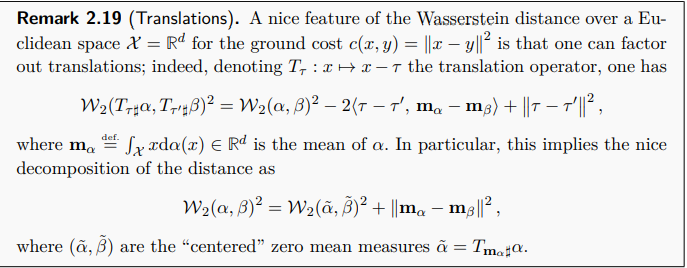
\includegraphics[width=0.7\linewidth]{images/WassAndTrans}
		\caption{https://arxiv.org/pdf/1803.00567. See Remark 2.31 for Wass distance between two Gaussians in $R^d$}
		\label{fig:wassandtrans}
	\end{figure}
	
	\begin{figure}
		\centering
		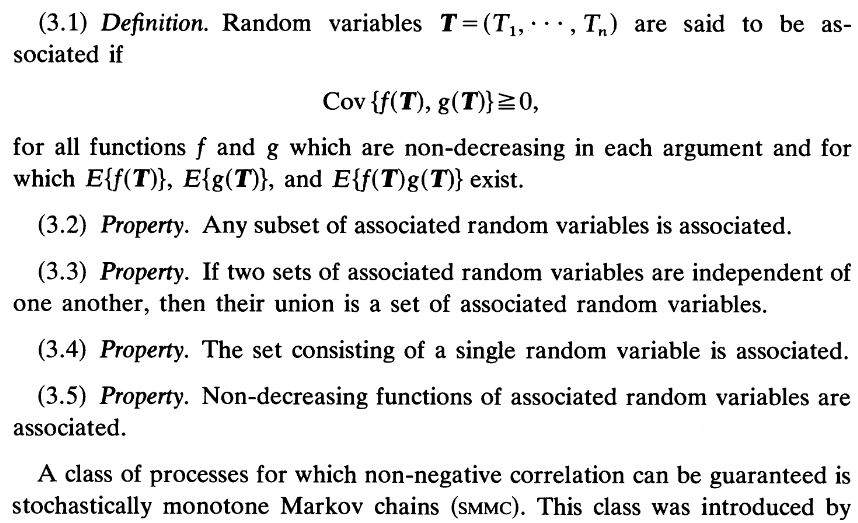
\includegraphics[width=0.7\linewidth]{images/associated}
		\caption{This is perhaps my only hope of extending \ref{thm:crngen} to $\mathbb{R}^d$. This paper says that when using CRN, variance is reduced. Could one somehow define functions to show that CRN actually generates the optimal reduction in covariance? Also, what does it mean for $f$ to be non-decreasing in each argument? (Comparing Stochastic Systems Using Regenerative Simulation with Common Random Numbers
			Philip Heidelberger, Donald L. Iglehart
			https://www.jstor.org/stable/1426860?seq=7)}
		\label{fig:associated}
	\end{figure}
	
	\begin{figure}
		\centering
		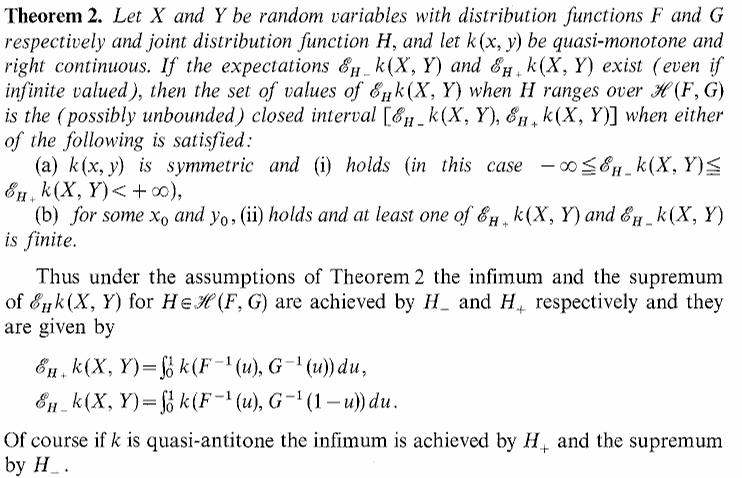
\includegraphics[width=0.7\linewidth]{images/original_wass_optimal}
		\caption{Something powerful is noted here: for any $H\in \mathcal{H}(\mathcal{L}(X), \mathcal{L}(Y))$, $E_{H}[k(X,Y)]\in [E_{H_+[X,Y]}, E_{H_-[X,Y]}]$. This set is convex and compact, but again only applies to $\mathbb{R}$}
		\label{fig:originalwassoptimal}
	\end{figure}
	
	\printbibliography
\end{document}
